\documentclass[12pt]{article}

\usepackage{graphicx}
\usepackage{amsmath}
\usepackage{amssymb}
\usepackage{natbib}
\usepackage{amsfonts}
\usepackage{multicol}
\usepackage{float}
\usepackage{oldgerm}
\usepackage{bm}
\usepackage{mathtools}
\usepackage{wrapfig}
\usepackage{fancyhdr}
\usepackage[export]{adjustbox}
\usepackage{xcolor}
\usepackage[shortlabels]{enumitem}

\pagestyle{empty}

\setlength{\headsep}{0.5cm}
\setlength{\oddsidemargin}{-0.5cm}
\setlength{\textwidth}{16.5cm}
\setlength{\textheight}{24cm}
\voffset = -2cm


\pagestyle{fancy}
\fancyhf{}
\rfoot{
\includegraphics[width=1.0in]{cnm.png}}
\lfoot{ENGR2910 - Final}
\setlength\parindent{0pt}
\begin{document}

\begin{center}
\hfil
{\large\bf {ENGR 2910-101: Circuit Analysis}}
\hfill Instructor: Brian Rashap\\
Final \hfill Due: 04/19/23\\
\hrulefill\\
\end{center}


{\bf Question 1} [15] 
\newline

Use source transformation to find the Thevenin equivalent with respect to terminals A and B for the circuit below, if:
\begin{itemize}
\item $V_g = 240 \angle 0^{\circ}$
\item $L_1 = j60 \Omega$
\item $C_1 = -j48 \Omega$
\item $R_1 = 36 \Omega$
\end{itemize}

\begin{figure}[h!]
\centering 
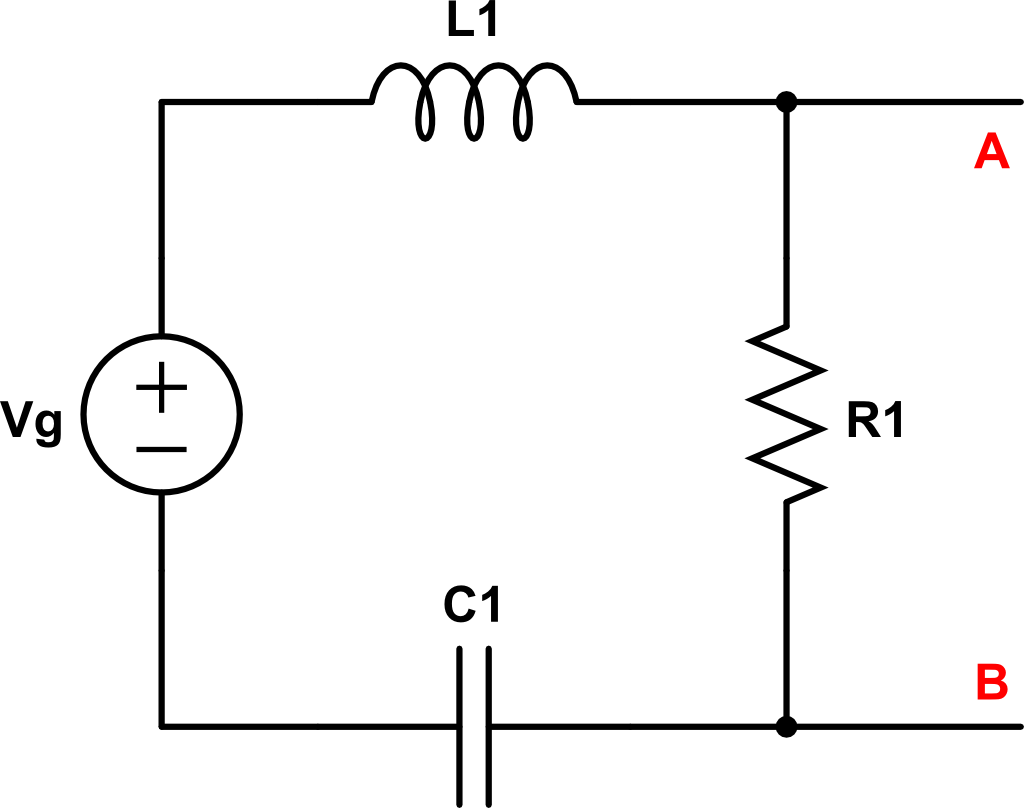
\includegraphics[clip,width=0.40\textwidth]{final_1.png}
\end{figure}

\newpage

{\bf Question 2} [15]
\newline

Find the value of R that makes the below circuit Critically Damped.

\begin{figure}[h!]
\centering 
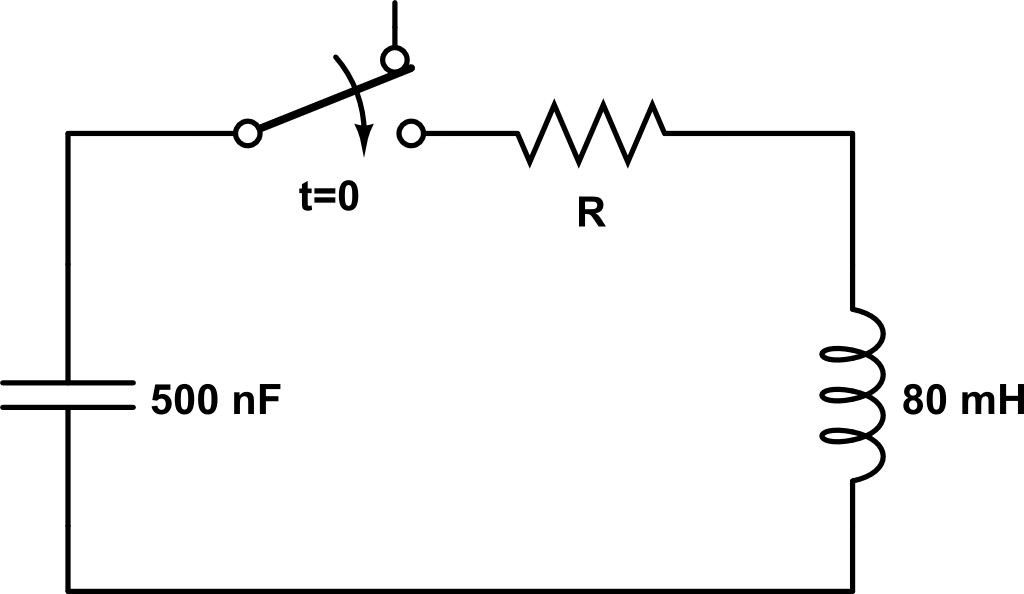
\includegraphics[clip,width=0.40\textwidth]{final_2.png}
\end{figure}

\newpage

{\bf Question 3} [15]
\newline

Use the Node-Voltage method to find the matrix representation of $V_1$ and $V_2$ if $i_g = 5 \cos{(2500t)} A$ and $v_g = 20\cos{(2500t+ 90^{\circ})} V$. You do NOT need to solve for $V_1$ and $V_2$, nor reduce the matrix to reduced row echelon form.

\begin{figure}[h!]
\centering 
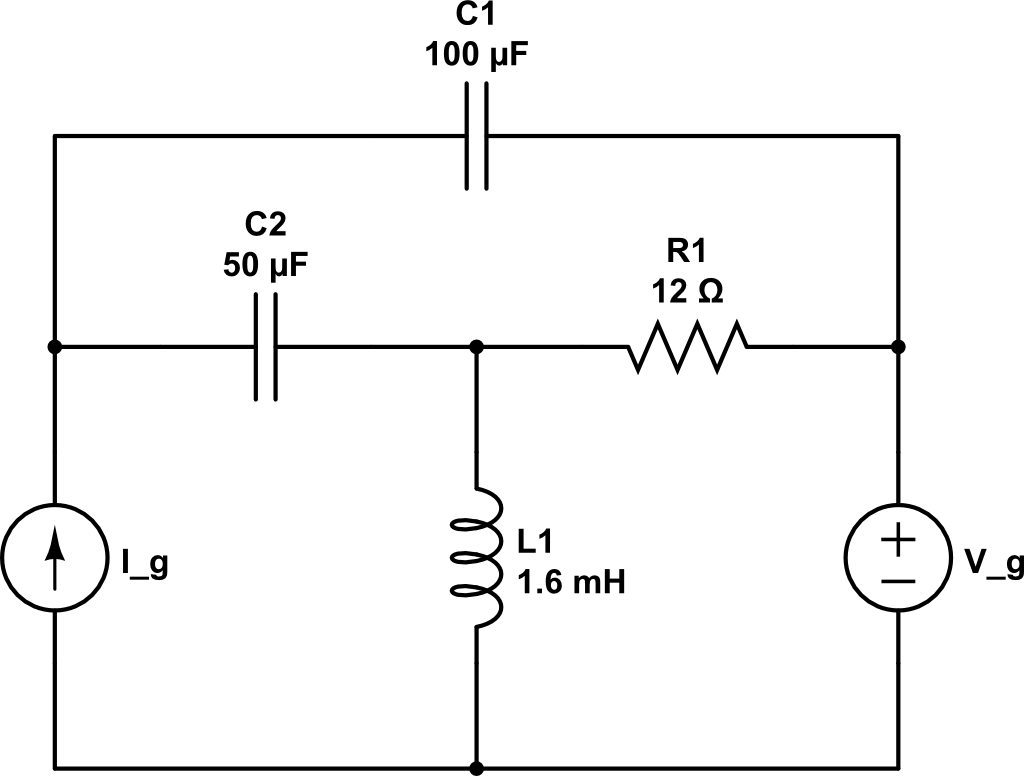
\includegraphics[clip,width=0.49\textwidth]{final_3.png}
\end{figure}

\newpage

{\bf Question 4} [15]
\newline

Find $Z_{eq}$ for the circuit below if
\begin{itemize}
\item $L_1 = j4 \Omega$
\item $L_2 = j20 \Omega$
\item $C_1 = -j8 \Omega$
\item $C_2 = -j20 \Omega$
\end{itemize}

\begin{figure}[h!]
\centering 
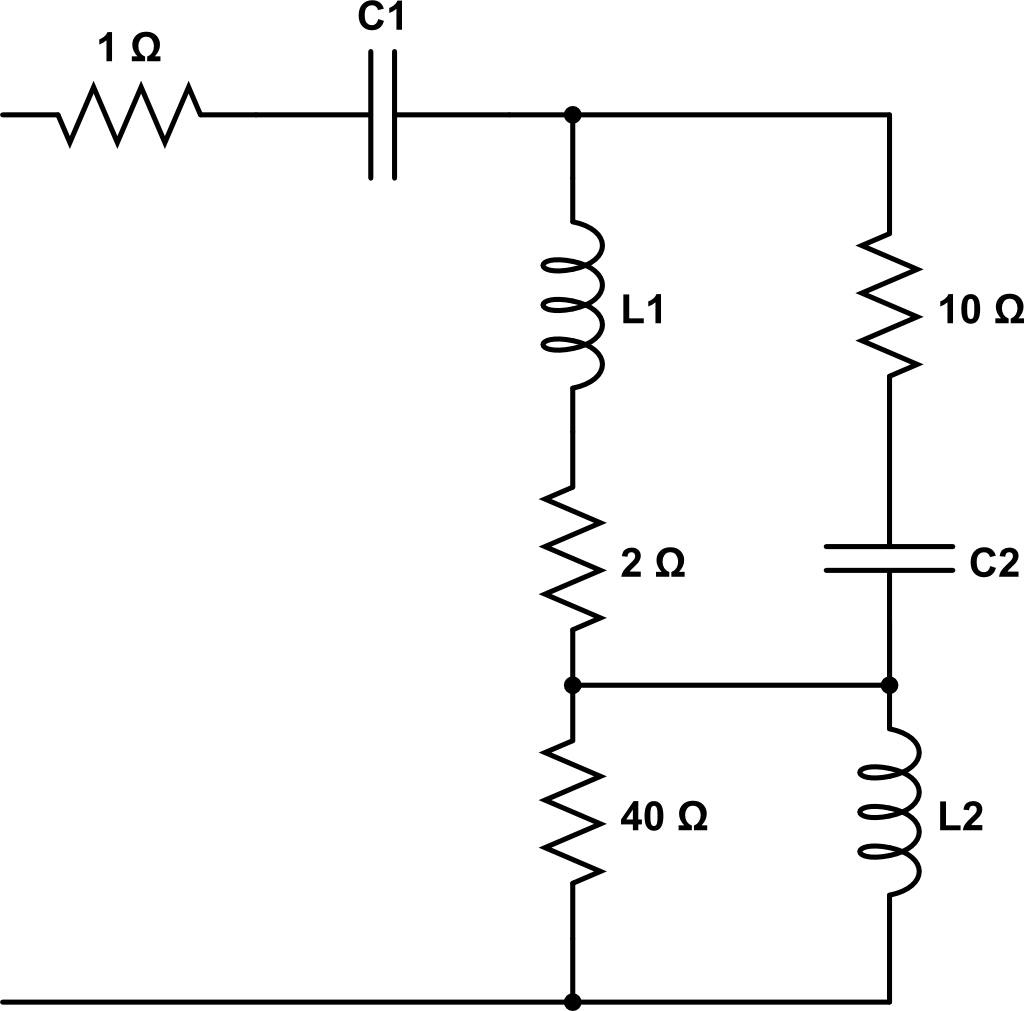
\includegraphics[clip,width=0.40\textwidth]{final_4.png}
\end{figure}

\newpage


{\bf Question 5} [20]
\newline

\begin{figure}[h!]
\centering 
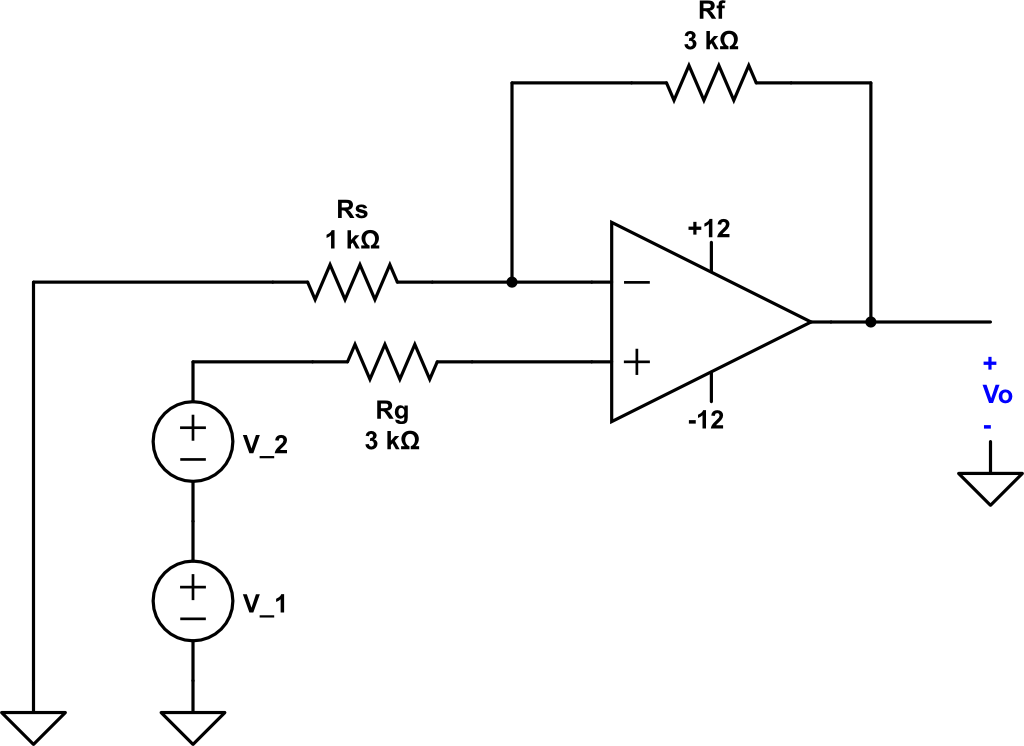
\includegraphics[clip,width=0.49\textwidth]{final_5.png}
\end{figure}

\begin{enumerate}[(a)]
\item What are the three Ideal Op Amp assumptions and their implications to voltages and currents in the circuit?
\item For the Op Amp Circuit above, use Kirchhoff's Laws to derive the gain.
\item If $v_1 = 1 V$ and $v_2 = 3 * \cos{(\frac{\pi}{2}t)}$, draw a graph of $v_o$. Show at least two periods of the output. 
\end{enumerate}

\newpage

{\bf Question 6} [20]
\newline

The two switches in the below circuit are synchronized. When the Switch 1 opens, Switch 2 closes, and vice versa. Switch 1 has been open for a long time before closing at $t=0$. Find $i_L(t)$ for $t \geq 0$. 

\begin{figure}[h!]
\centering 
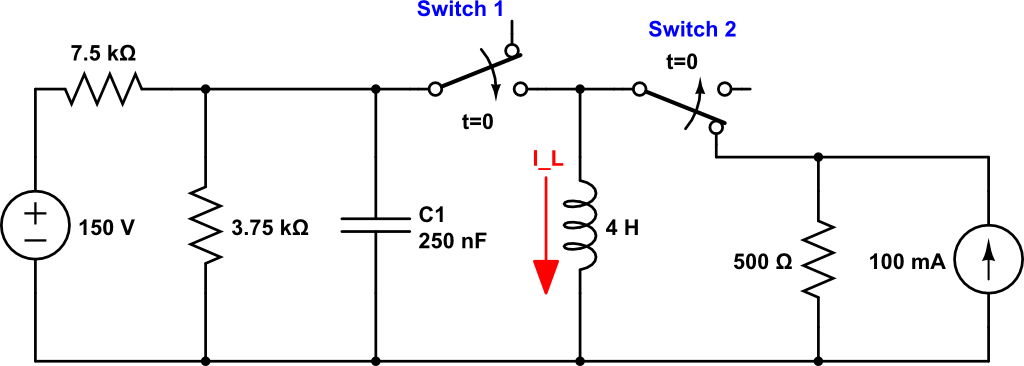
\includegraphics[clip,width=0.72\textwidth]{final_6.png}
\end{figure}

\end{document}
